\documentclass[11pt, aspectratio=169]{beamer}

% Підтримка української мови та кирилиці
\usepackage[T2A]{fontenc}
\usepackage[utf8]{inputenc}
\usepackage[ukrainian]{babel}
\usepackage{amsmath, amssymb}
\usepackage{graphicx} % Для відображення картинок

% Налаштування теми презентації
\usetheme{Madrid}
\usecolortheme{whale}
\setbeamertemplate{navigation symbols}{}

\title[Барицентрична інтерполяція]{Дослідження та програмна реалізація методу масштабування зображень з використанням барицентричної формули на основі вузлів інтерполяції Чебишева}
\author{
	Липянчик Євген \\
	{\small Науковий керівник: к.~ф.-м.~н Хребет~В.~Г.} \\
	{\small Нормоконтролер: Василик~В.~Б.}
}
\institute{Державний університет «Київський авіаційний інститут»}
\date{2026}

\begin{document}
	
	% --- Слайд 1: Титульний ---
	\begin{frame}
		\titlepage
	\end{frame}
	
	% --- Слайд 2: Формулювання теми та актуальність ---
	\begin{frame}{Формулювання теми та актуальність}
		\begin{itemize}
			\item Задачі масштабування зображень є критично важливими у сферах геоінформаційних систем (ГІС), обробки супутникових знімків, медичної візуалізації та комп'ютерного зору.
			\item Від вибору алгоритму масштабування безпосередньо залежить баланс між обчислювальною складністю та якістю зображення.
			\item Більшість класичних методів інтерполяції використовують рівномірні сітки та розглядають лише локальну інтерполяцію.
			\item \textbf{Новизна підходу:} використання нестандартного моделювання із застосуванням нерівномірних сіток дискретизації, що складаються з точок екстремумів поліномів Чебишева другого роду.
			\item Метод гнучко працює як у напрямку зменшення, так і збільшення зображень для великих коефіцієнтів.
		\end{itemize}
	\end{frame}
	
	\begin{frame}{постановка задачі}
		\begin{enumerate}
			\item Ознайомитися з існіючими методами масштабування зображень.
			\item  Адаптувати математичку модель цифрового зображення на нерівномірних сітках для випадку вузлів Чебишева другого роду.
			\item Поширити другу барицентричну формулу на двовимірний випадок.
			\item Розробити програмне забезпечення для масштабування зображень використовуючи новий запропонований та стандартні реалізовані методи.
			\item Провести тестування та порівняльний аналіз результатів роботи розробленого алгоритму з класичними методами масштабування зображень.
		\end{enumerate}
	\end{frame}
	
	\begin{frame}{Класифікація візуальних артефактів масштабування}
		\begin{itemize}
			\item \textbf{Ефект дзвону (Ringing)} – поява одиночної паразитної хвилі поблизу різких меж зображення.
			\item \textbf{Перерегулювання (Overshooting)} – виникнення серії паразитних хвиль навколо контрастних переходів.
			\item \textbf{Субпіксельний зсув (Sub-pixel shift)} – небажана просторова трансляція всього зображення. 
			\item \textbf{Аліасинг (Aliasing)} – «східчастий ефект» на діагональних контурах. 
			\item \textbf{Розмиття (Blurring)} – втрата чіткості та різкості після масштабування.
		\end{itemize}
		\vspace{0.3cm}
	\end{frame}

	\begin{frame}{Базові методи просторового масштабування}
		\begin{itemize}
			\item \textbf{Інтерполяція за найближчим сусідом (Nearest Neighbor):} 
			\begin{itemize}
				\item \textit{Принцип:} Просте дублювання значення геометрично найближчого пікселя вихідного зображення.
				\item \textit{Особливості:} Найвища швидкість $\mathcal{O}(1)$, але виражена ступінчастість контурів (\textit{aliasing}).
			\end{itemize}
			
			\vspace{0.3cm}
			\item \textbf{Білінійна інтерполяція (Bilinear):}
			\begin{itemize}
				\item \textit{Принцип:} Обчислення нового значення як зваженої суми чотирьох найближчих пікселів (окіл $2 \times 2$).
				\item \textit{Особливості:} Згладжує зубчасті краї, але призводить до відчутного розмиття (\textit{blurring}) різких границь.
			\end{itemize}
			
			\vspace{0.3cm}
			\item \textbf{Бікубічна інтерполяція (Bicubic):}
			\begin{itemize}
				\item \textit{Принцип:} Побудова гладких кубічних поверхонь на основі 16 сусідніх пікселів (окіл $4 \times 4$).
				\item \textit{Особливості:} Краще зберігає деталі, проте є ресурсомісткою і схильною до паразитних осциляцій (\textit{ringing artifacts}) на контрастних переходах.
			\end{itemize}
		\end{itemize}
	\end{frame}

\begin{frame}{Вузли Чебишева другого роду}
	\begin{figure}[htbp]
		\centering
		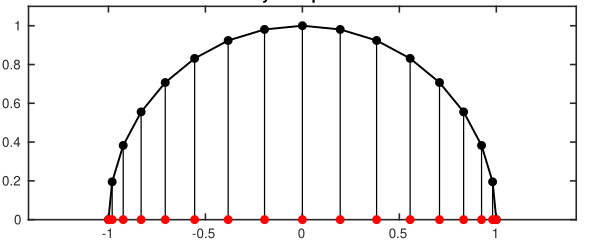
\includegraphics[width=0.6\textwidth]{chebPoints}
		\caption{Точки Чебишева}
	\end{figure}
	
	\begin{equation}
		x_j = \cos\left(\frac{j\pi}{n}\right), \qquad 0 \le j \le n.
	\end{equation}
	
\end{frame}
	
	\begin{frame}{Порівняння рівномірної та чебишевської сіток}
		\begin{columns}[t]
			\begin{column}{0.48\textwidth}
				\begin{figure}[htbp]
					\centering
					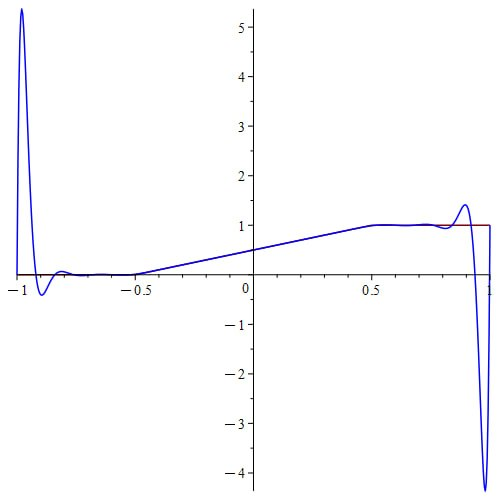
\includegraphics[width=0.7\linewidth]{uni}
					\caption{Поліноміальна інтерполяція на рівномірній сітці вузлів}
				\end{figure}
			\end{column}
			
			\hfill
			
			\begin{column}{0.48\textwidth}
				\begin{figure}[htbp]
					\centering
					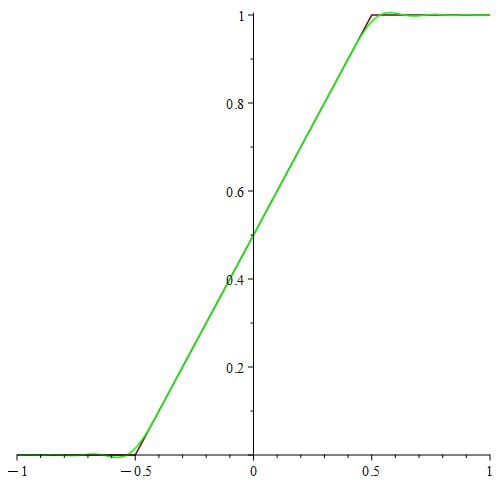
\includegraphics[width=0.7\linewidth]{cheb}
					\caption{Поліноміальна інтерполяція за вузлами Чебишева}
				\end{figure}
			\end{column}
		\end{columns}
	\end{frame}
	
		\begin{frame}{Математична модель: Барицентрична інтерполяція}
		\small % Зменшуємо розмір шрифту, щоб усі формули помістилися
		
		\textbf{Вузли Чебишева:}
		\begin{equation*}
			\omega_x = \left\{x_i = -\cos \frac{\pi i}{n}, i = \overline{0,n}\right\}, \quad \omega_y = \left\{y_j = -\cos \frac{\pi j}{m}, j = \overline{0,m}\right\}
		\end{equation*}
		
		\textbf{Барицентрична формула:}
		\begin{equation*}
			L_{n,m}(x_r, y_r) = \frac{\sideset{}{'}\sum_{i=0}^{n} \sideset{}{'}\sum_{j=0}^{m} \frac{(-1)^{i+j}}{(x_r-x_i)(y_r-y_j)} f_{ij}}{\sideset{}{'}\sum_{i=0}^{n} \sideset{}{'}\sum_{j=0}^{m} \frac{(-1)^{i+j}}{(x_r-x_i)(y_r-y_j)}}
		\end{equation*}
		
		\textbf{Символ $\sum'$ означає:}
		\begin{equation*}
			\sideset{}{'}\sum_{p=0}^{N} a_p = \frac{1}{2} a_0 + \sum_{p=1}^{N-1} a_p + \frac{1}{2} a_N
		\end{equation*}
	\end{frame}
	
\begin{frame}{Математична декомпозиція та оптимізація обчислень}
	\begin{block}{Декомпозиція ядра}
		Двовимірний барицентричний інтерполянт розкладається на два послідовні одновимірні проходи:
		\begin{equation}
			L_{n,m}(x, y) = \frac{\sideset{}{'}\sum\limits_{i=0}^{n} \dfrac{(-1)^{i}}{x - x_i}\, R_i(y)}{\sideset{}{'}\sum\limits_{i=0}^{n} \dfrac{(-1)^{i}}{x - x_i}}, \quad \text{де } 
			R_i(y) = \frac{\sideset{}{'}\sum\limits_{j=0}^{m} \dfrac{(-1)^{j}}{y - y_j}\, f_{ij}}{\sideset{}{'}\sum\limits_{j=0}^{m} \dfrac{(-1)^{j}}{y - y_j}}
		\end{equation}
	\end{block}
	
	\vspace{0.5cm}
	\textbf{Ключові інженерні рішення:}
	\begin{itemize}
		\item \textbf{Кешування ваг:} Одноразовий розрахунок матриць \texttt{W\_X} та \texttt{W\_Y} у паралельних потоках.
		\item \textbf{Безблокова паралелізація обчислень:} Розпаралелювання двопрохідної інтерполяції.
	\end{itemize}
\end{frame}

\begin{frame}{Матрична форма та двопрохідне обчислення}
	\begin{block}{Фінальне матричне рівняння (Декомпозиція)}
		\vspace{-0.1cm}
		\begin{equation*}
			\mathbf{G} = \mathbf{B}\, \mathbf{F}\, \mathbf{A}^{\top}
		\end{equation*}
	\end{block}
	
	\vspace{0.2cm}
	\textbf{Двопрохідна схема обчислень:}
	\begin{enumerate}
		\item \textbf{Перший прохід} (інтерполяція вздовж $y$): 
		\begin{equation*}
			\mathbf{T} = \mathbf{B}\, \mathbf{F}, \quad \mathbf{T} \in \mathbb{R}^{H_2 \times W}
		\end{equation*}
		\item \textbf{Другий прохід} (інтерполяція вздовж $x$): 
		\begin{equation*}
			\mathbf{G} = \mathbf{T}\, \mathbf{A}^{\top}, \quad \mathbf{G} \in \mathbb{R}^{H_2 \times W_2}
		\end{equation*}
	\end{enumerate}
	
	\vspace{0.1cm}
	\textbf{Переваги матричного представлення:}
	\begin{itemize}
		\item \textbf{Розділення задач:} Геометричні матриці ваг $\mathbf{A}$ та $\mathbf{B}$ розраховуються один раз і не залежать від колірних значень пікселів.
		\item \textbf{Апаратна сумісність:} Алгоритм зводиться до множення матриць що відкриває шлях для використання оптимізованих бібліотек лінійної алгебри.
	\end{itemize}
\end{frame}
	
\begin{frame}{Програмна оптимізація матричного методу за допомогою OpenCV}
	\begin{block}{Поканальне оптимізоване множення (\texttt{cv::gemm})}
		\vspace{-0.1cm}
		\begin{equation*}
			\mathbf{G}_c = \mathbf{B} \cdot \mathbf{F}_c \cdot \mathbf{A}^{\top}, \quad c \in \{R, G, B\}
		\end{equation*}
	\end{block}
	
	\vspace{0.1cm}
	\textbf{Чинники апаратного прискорення OpenCV:}
	\begin{enumerate}
		\item \textbf{Векторизація обчислень (SIMD):} Автоматичне використання інструкцій SSE, AVX/AVX2 для обробки кількох елементів за один такт процесора.
		\item \textbf{Кеш-оптимізація:} Блокове множення (\textit{block matrix multiplication}) під розміри кешу L1/L2 для мінімізації звернень до RAM.
		\item \textbf{Прихована багатопотоковість:} Автоматичне розпаралелювання операцій через вбудовані інструменти (Intel TBB, OpenMP або Apple GCD).
	\end{enumerate}
\end{frame}

\begin{frame}{Локальна барицентрична інтерполяція}
	\textbf{Проблема:} Глобальна інтерполяція може породжувати феномен Гіббса що проявляэться як осциляції на різких межах.
	
	\begin{block}{Рішення: Метод локальної інтерполяції}
		Замість єдиного глобального полінома будується локальний інтерполянт низького степеня в околі $K \times K$ пікселів.
	\end{block}
	
	\vspace{0.4cm}
	\textbf{Властивості алгоритму:}
	\begin{itemize}
		\item \textbf{Швидкодія:} Обчислювальна складність є суворо лінійною — $\mathcal{O}(W_2 \cdot H_2)$.
		\item \textbf{Керування артефактами (розмір вікна $K$):}
		\begin{itemize}
			\item $\mathbf{K = 3}$  — ідеально різкі краї, повне придушення осциляцій.
			\item $\mathbf{K \ge 5}$ — вища точність на градієнтах, але з ризиком мікро-осциляцій.
		\end{itemize}
	\end{itemize}
\end{frame}

	
	% --- Слайд 4: Інтерфейс ---
\begin{frame}{Інтерфейс програми та процес роботи (1/2)}
	\begin{columns}
		\begin{column}{0.5\textwidth}
			\centering
			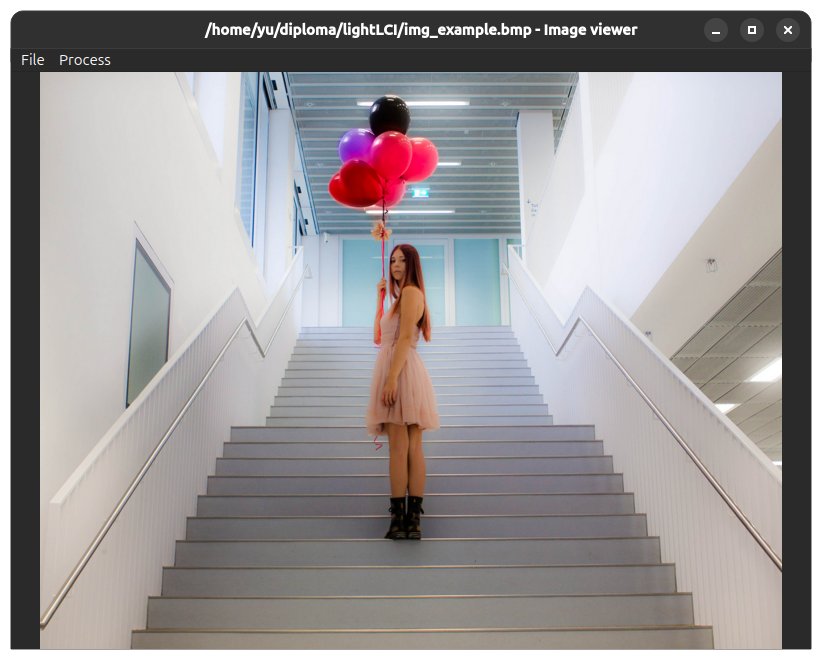
\includegraphics[width=0.95\linewidth]{main} \\
			\vspace{0.3cm}
			\large 1. Завантаження вихідного зображення
		\end{column}
		\begin{column}{0.5\textwidth}
			\centering
			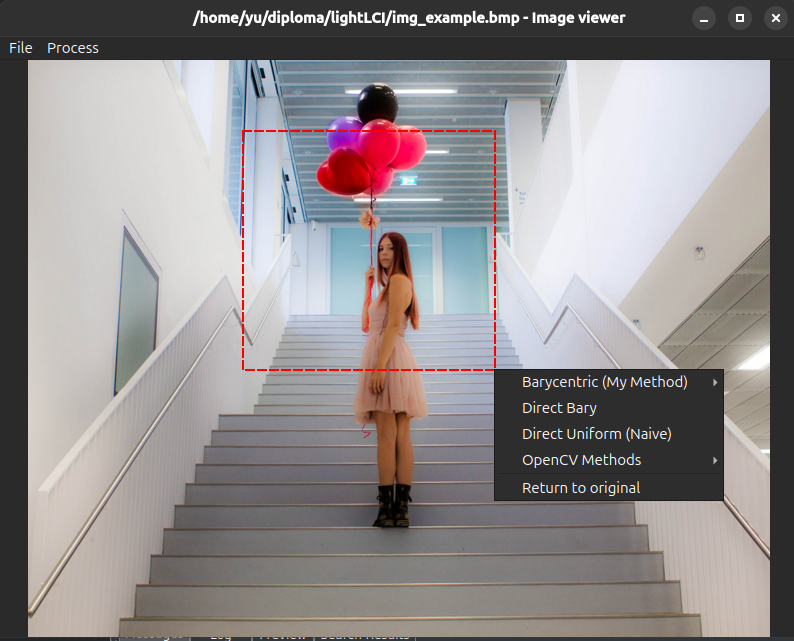
\includegraphics[width=0.95\linewidth]{menu} \\
			\vspace{0.3cm}
			\large 2. Виділення області та вибір методу
		\end{column}
	\end{columns}
\end{frame}

% --- Слайд 5: Інтерфейс (Частина 2) ---
\begin{frame}{Інтерфейс програми та процес роботи (2/2)}
	\begin{columns}
		\begin{column}{0.5\textwidth}
			\centering
			% Збільшив ширину віконця коефіцієнта, оскільки тепер є місце
			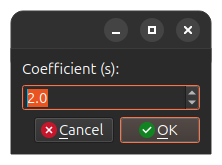
\includegraphics[width=0.55\linewidth]{coef} \\
			\vspace{0.3cm}
			\large 3. Задання коефіцієнта масштабування
		\end{column}
		\begin{column}{0.5\textwidth}
			\centering
			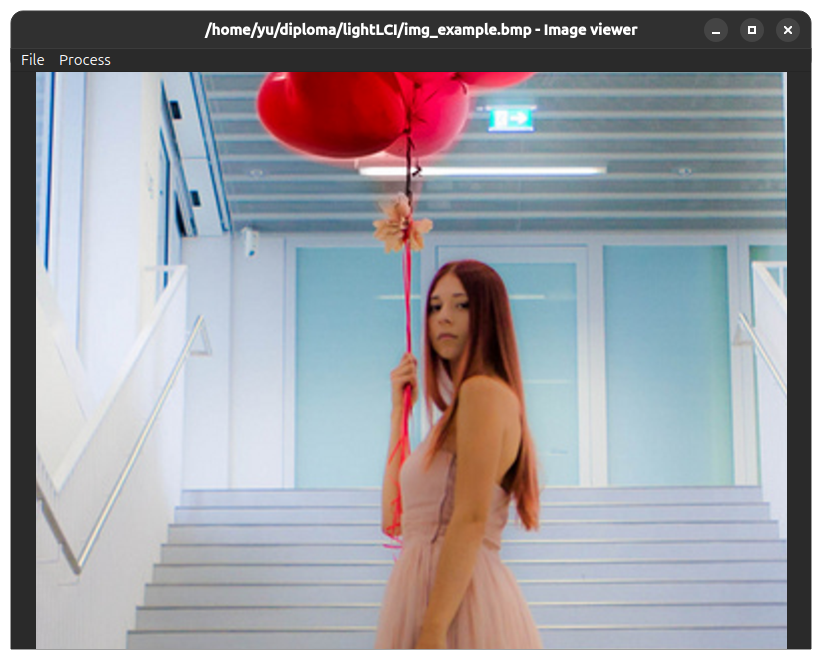
\includegraphics[width=0.95\linewidth]{result} \\
			\vspace{0.3cm}
			\large 4. Результат роботи барицентричного методу
		\end{column}
	\end{columns}
\end{frame}
	
\begin{frame}{Методологія тестування масштабування}
	\begin{center}
		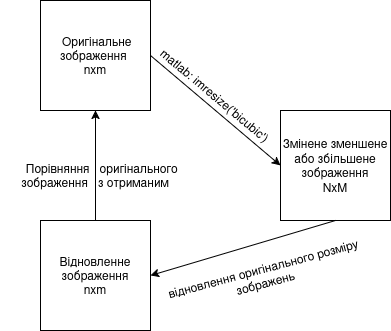
\includegraphics[width=0.55\linewidth]{TestDiagram.drawio.png} \\
	\end{center}
\end{frame}
	
	\begin{frame}{Графычний ынтерфейс тестування}
		\begin{center}
			
		\end{center}
	\end{frame}
	% --- Слайд 6: Висновки ---
	\begin{frame}{Висновки}
		\begin{itemize}
			\item Представлено новий підхід до масштабування на основі глобальної інтерполяції за допомогою двовимірного інтерполяційного полінома Чебишева.
			\item \textbf{Подальший розвиток:} Оптимізація алгоритму для отримання найкращих результатів по часу розрахунків та повна автоматизація розрахунку порівняльних характеристик.
		\end{itemize}
	\end{frame}
	
\end{document}